\documentclass[tikz,border=10pt]{standalone}
\usepackage{tikz}
\usetikzlibrary{calc, intersections}

\begin{document}
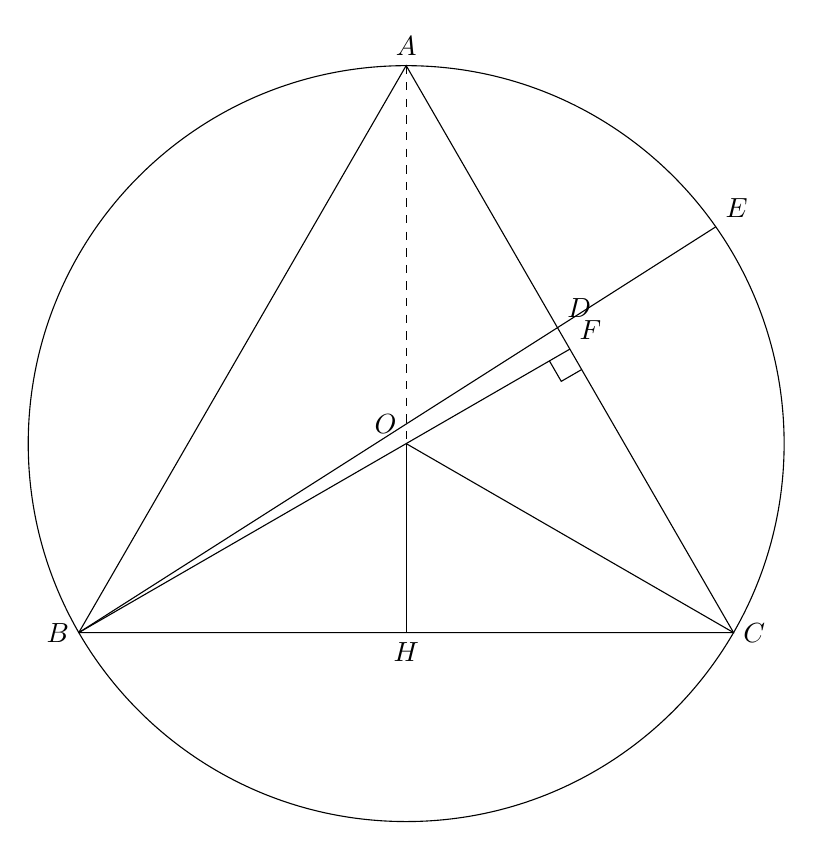
\begin{tikzpicture}[scale=1.2]
    % Define coordinates
    \coordinate (O) at (0,0);
    \coordinate (A) at (0,4);
    \coordinate (B) at ({4*cos(210)}, {4*sin(210)}); % approx (-3.46, -2)
    \coordinate (C) at ({4*cos(330)}, {4*sin(330)}); % approx (3.46, -2)
    \coordinate (H) at (0,-2);
    
    % F is midpoint of AC (since triangle is equilateral-ish and BF passes through O)
    \coordinate (F) at ($(A)!0.5!(C)$);
    
    % E is on the circle, angle 35 degrees
    \coordinate (E) at ({4*cos(35)}, {4*sin(35)});
    
    % D is intersection of BE and AC
    \path [name path=BE] (B) -- (E);
    \path [name path=AC] (A) -- (C);
    \path [name intersections={of=BE and AC, by=D}];
    
    % Draw Circle
    \draw (O) circle (4);
    
    % Draw Triangle ABC
    \draw (A) -- (B) -- (C) -- cycle;
    
    % Draw AH (dashed AO, solid OH)
    \draw[dashed] (A) -- (O);
    \draw (O) -- (H);
    
    % Draw Radii/Segments from O
    \draw (O) -- (C);
    % Note: OB is part of BF, drawn below
    
    % Draw BF (Altitude/Median passing through O)
    \draw (B) -- (F);
    
    % Draw BE (Chord)
    \draw (B) -- (E);
    
    % Right angle mark at F
    % Vector FC
    \coordinate (vecFC) at ($(C)-(F)$);
    \coordinate (vecFB) at ($(B)-(F)$);
    % Normalize roughly for drawing
    \draw ($(F)!0.25cm!(C)$) -- ($(F)!0.25cm!(C) + ($(F)!0.25cm!(B)$) - (F)$) -- ($(F)!0.25cm!(B)$);
    
    % Labels
    \node[above] at (A) {$A$};
    \node[left] at (B) {$B$};
    \node[right] at (C) {$C$};
    \node[above right] at (D) {$D$};
    \node[above right] at (E) {$E$};
    \node[above right] at (F) {$F$};
    \node[below] at (H) {$H$};
    \node[above left] at (O) {$O$};
    
\end{tikzpicture}
\end{document}
